\chapter{Introduction}
\section{Overview}
Owning a computer was the new thing in the world. Everyone wanted to have one. The first computers were very large in size but as the years passed by, the size decreased. We now have portable computers. Computers may crash and we lose all our data, or the computation we want to perform, our computers cannot handle. A need arose to increase storage space and processing power. We would not always be purchasing new machines and training staff all the time as the needs changed everyday.  Thus we required to store and process our data elsewhere in addition to the local storage. This was characterized by Cloud Computing. Cloud Computing can be described as using the cloud (some server stored somewhere anonymous) to carry out tasks like storage and data management over a network rather than doing it in our own computers.  

We enjoyed cloud computing for a while but then the issue of security came along. A user does not have control of whom would access his/her data while in the cloud. Mischievous users may intentionally or accidentally get hold of someone else's data. One can imagine a leakage of a patient's examination results or diagnoses. It started by using for example a symbol to represent a patient. Yes the patient's name may be anonymous, but if someone has access to the hospital's data, they would know how many people are suffering from a certain disease among others. This user can decide to cause unnecessary chaos or theft in case of a bank where a customer's personal information such as credit card pin code is accessed. It became possible to encrypt data and store it but performing computations on this encrypted data was not possible. Encryption is simply using a different representation of data for instance using 123 to represent the word transform. Only someone who knows how to interpret it can use it.
 
Homomorphic Encryption shows that it is actually possible to perform computations on encrypted data.

\section{Background and Motivation} 
In April 2011, a Play Station's network owned by Sony was hacked. There was exposure of customers information like credit card and passwords. The responsibility for this incidence was accepted by Sony. They realized that they had not done enough to ensure security of their customers' data. They would have encrypted it before storage. In this same period researchers also discovered that files in Dropbox were stored unencrypted. This lead to users leaving and closing their accounts with Dropbox since they felt insecure.  

According to, ensuring security would be done at different levels. Securing the hardware (this is the physical system), software (set of instructions executed in the system) and the data itself. In the hardware, locks were put to limit access to unauthorized persons. Systems to detect an intrusion and devices that verify persons identity were put into place. In the software, programs that limit access to database and protect one user from other users were developed. Also, software programs were written in such a way that their weaknesses could not be easily exploited. Password checkers and virus scanners application programs were also developed. The solution to the data was encryption. Data is only useful to parties if it can be readable and interpreted. Encrypted data is only useful if one can decrypt it.  All this assured the user of security. At the instances where the user needed to use the data then there was a problem because the data needed to be decrypted before any form of computations. This raised a security issue again. We needed to develop a system that allows computations on encrypted data. This is known as Homomorphic Encryption. This assured the user of total security. 

Previous works have been done trying to explain how Homomorphic Encryption can be implemented on various platforms using different types of data. In 2013  tried to explain a model which encrypts hospital data. After the computations are done the number of patients suffering from a certain disease is returned in an encrypted format. The hospital's management then decrypts it. Showed a system where different people are using it to perform an optimization problem among themselves. An optimization problem is a problem where you want the output to be the maximum based on certain inputs, for example maximum profit. The task is to find the inputs. These people work without revealing any information about their inputs to the server. Using a similar approach to these works, we will discuss possible applications of Quantum Homomorphic Encryption using example use cases.


\section{Aim and Objectives of the Study}
Imagine you own a business and you want to charge different prices to different people based on their financial capabilities and customer loyalty. Your resources are limited thus you have to outsource resources such as storage. You do not want this information to leak to the public since this may make some customers to withdraw. You want to maintain the privacy of this information. The system should be able to determine the financial status and loyalty of a customer then charge accordingly. No information about the customer is revealed or the prices charged to other customers.

The aim of this essay is to show the current state of security while requiring services from an untrusted server. The objectives include explaining vividly the security concerns and showing steps taken to counter these issues. This is done by discussing about classical computing with its limitations compared to quantum computing. We will also see the different ideas quantum computing brings about which makes it attractive compared to classical computing, the process of Quantum Homomorphic Encryption in details and application examples.

\section{Purpose of the Study}
There was a time when bank robbery was the order of the day. Banks solved this issue by putting so many security measures such as several locks and authentication before accessing where the actual money was. Banks also required several people to approve before large transactions were made. In 2017, three men dug a tunnel for six months into a Kenyan bank and made away with 50 million Kenyan shillings which is approximately 500,000 US dollars. This shows that security issues cannot be solved 100 percent. A determined person will always find a loophole. How can we ensure that the loopholes are not easily discovered and exploited?

The purpose of this essay is to show how computing security has evolved over the years, the steps and measures taken in different settings using the resources available, the plans under way to secure the data and computing in future and the new discoveries especially Quantum Computing and its effect on computing security. We will also see why one would consider a Quantum Homomorphic Encryption over a Classical Homomorphic Encryption. 

\section{Organization of Essay}

This essay is subdivided into five different chapters. In Chapter 2 we will discuss about classical and cloud computing with their limitations compared to quantum computing. In Chapter 3, quantum computing is vividly discussed. Different types of encryption in quantum computing and why one is chosen over the other are also discussed. Chapter 4 talks about examples of use cases where Quantum Homomorphic Encryption could be used. Chapter 5 contains the conclusion with recommendations.

%Explain the context of your essay topic, so that the
%topic itself appears motivated, natural and important.
%
%\begin{figure}[h]
%\psfrag{A}{$d^2$}
%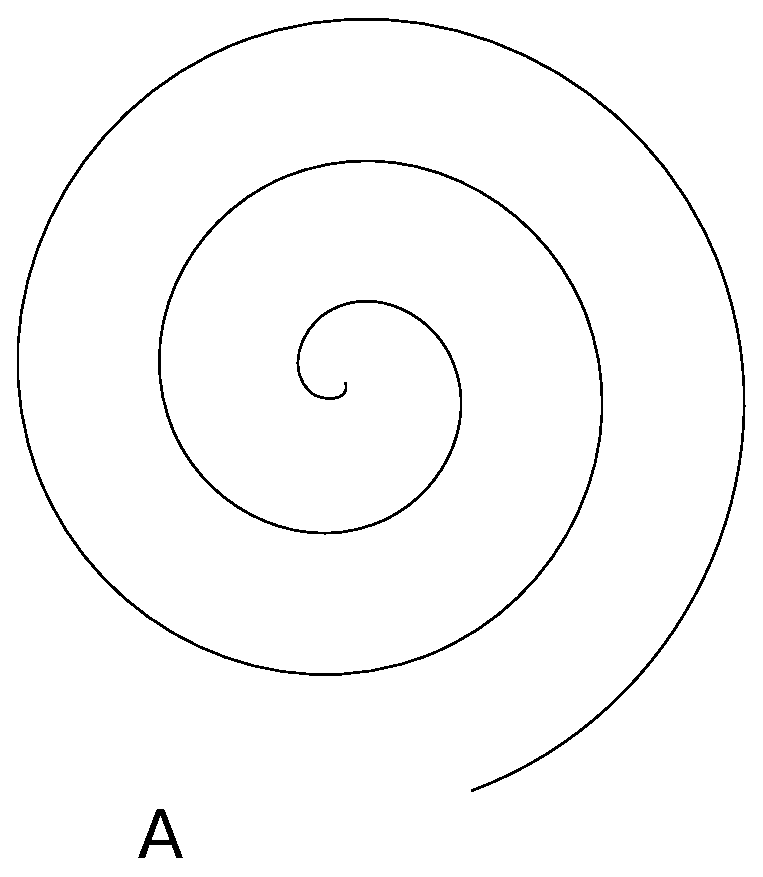
\includegraphics[scale=0.5]{images/drawing.eps}
%\end{figure}
%
%Paragraphs are separated by blank lines in the \LaTeX\ code, 
%and the line spacing, paragraph indentation,
%and paragraph spacing are set in the preamble for you, 
%according to AIMS house style.
%
%This is a textual citation \citet{shannon44}. And this is a parenthetical citation \citep{shannon44}. You probably want to use the latter more often.
%
%\section{Moving On}
%Let's demonstrate a figure by looking at Fig.~\ref{bandwidth}. 
%
%\begin{figure}[!h]
%% Use "\centering" in floats (figure, table), but if you need to center
%% some text (why?) use "\begin{center}...\end{center}".
%\centering 
%% Figure environments same as 0.8 * \textwidth please
%% That does not necessarily mean the actual picture size,
%% it is a guideline for the environment which could contain
%% 2 or more pictures! Be consistent and follow the guidelines
%% provided in your sources.
%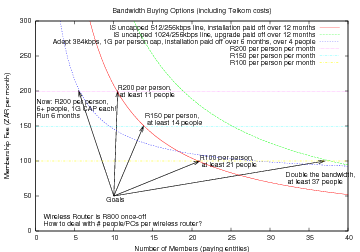
\includegraphics[width=0.8\textwidth]{images/bandwidth-colour.png}
%\caption{Planning community bandwidth sharing costs. 
%  Note caption capitalization.}
%\label{bandwidth} 
%% if you move the label it breaks the reference numbering; 
%% always have it *after* the caption.
%\end{figure}
%
%Remember how to include code with {\tt verbatim} 
%and to fix the tabs in {\sf python} in a verbatim environment? 
%It may be best to have an `include' command for code, 
%not to have to re-edit it all the time.
%\verbatimtabinput{code/mycode.py}
%
%
